\documentclass[11pt,preprint, authoryear]{elsarticle}

\usepackage{lmodern}
%%%% My spacing
\usepackage{setspace}
\setstretch{1.2}
\DeclareMathSizes{12}{14}{10}{10}

% Wrap around which gives all figures included the [H] command, or places it "here". This can be tedious to code in Rmarkdown.
\usepackage{float}
\let\origfigure\figure
\let\endorigfigure\endfigure
\renewenvironment{figure}[1][2] {
    \expandafter\origfigure\expandafter[H]
} {
    \endorigfigure
}

\let\origtable\table
\let\endorigtable\endtable
\renewenvironment{table}[1][2] {
    \expandafter\origtable\expandafter[H]
} {
    \endorigtable
}


\usepackage{ifxetex,ifluatex}
\usepackage{fixltx2e} % provides \textsubscript
\ifnum 0\ifxetex 1\fi\ifluatex 1\fi=0 % if pdftex
  \usepackage[T1]{fontenc}
  \usepackage[utf8]{inputenc}
\else % if luatex or xelatex
  \ifxetex
    \usepackage{mathspec}
    \usepackage{xltxtra,xunicode}
  \else
    \usepackage{fontspec}
  \fi
  \defaultfontfeatures{Mapping=tex-text,Scale=MatchLowercase}
  \newcommand{\euro}{€}
\fi

\usepackage{amssymb, amsmath, amsthm, amsfonts}

\def\bibsection{\section*{References}} %%% Make "References" appear before bibliography


\usepackage[round]{natbib}

\usepackage{longtable}
\usepackage[margin=2.3cm,bottom=2cm,top=2.5cm, includefoot]{geometry}
\usepackage{fancyhdr}
\usepackage[bottom, hang, flushmargin]{footmisc}
\usepackage{graphicx}
\numberwithin{equation}{section}
\numberwithin{figure}{section}
\numberwithin{table}{section}
\setlength{\parindent}{0cm}
\setlength{\parskip}{1.3ex plus 0.5ex minus 0.3ex}
\usepackage{textcomp}
\renewcommand{\headrulewidth}{0.2pt}
\renewcommand{\footrulewidth}{0.3pt}

\usepackage{array}
\newcolumntype{x}[1]{>{\centering\arraybackslash\hspace{0pt}}p{#1}}

%%%%  Remove the "preprint submitted to" part. Don't worry about this either, it just looks better without it:
\makeatletter
\def\ps@pprintTitle{%
  \let\@oddhead\@empty
  \let\@evenhead\@empty
  \let\@oddfoot\@empty
  \let\@evenfoot\@oddfoot
}
\makeatother

 \def\tightlist{} % This allows for subbullets!

\usepackage{hyperref}
\hypersetup{breaklinks=true,
            bookmarks=true,
            colorlinks=true,
            citecolor=blue,
            urlcolor=blue,
            linkcolor=blue,
            pdfborder={0 0 0}}


% The following packages allow huxtable to work:
\usepackage{siunitx}
\usepackage{multirow}
\usepackage{hhline}
\usepackage{calc}
\usepackage{tabularx}
\usepackage{booktabs}
\usepackage{caption}


\newenvironment{columns}[1][]{}{}

\newenvironment{column}[1]{\begin{minipage}{#1}\ignorespaces}{%
\end{minipage}
\ifhmode\unskip\fi
\aftergroup\useignorespacesandallpars}

\def\useignorespacesandallpars#1\ignorespaces\fi{%
#1\fi\ignorespacesandallpars}

\makeatletter
\def\ignorespacesandallpars{%
  \@ifnextchar\par
    {\expandafter\ignorespacesandallpars\@gobble}%
    {}%
}
\makeatother

\newenvironment{CSLReferences}[2]{%
}

\urlstyle{same}  % don't use monospace font for urls
\setlength{\parindent}{0pt}
\setlength{\parskip}{6pt plus 2pt minus 1pt}
\setlength{\emergencystretch}{3em}  % prevent overfull lines
\setcounter{secnumdepth}{5}

%%% Use protect on footnotes to avoid problems with footnotes in titles
\let\rmarkdownfootnote\footnote%
\def\footnote{\protect\rmarkdownfootnote}
\IfFileExists{upquote.sty}{\usepackage{upquote}}{}

%%% Include extra packages specified by user
\usepackage{booktabs}
\usepackage{caption}
\usepackage{longtable}

%%% Hard setting column skips for reports - this ensures greater consistency and control over the length settings in the document.
%% page layout
%% paragraphs
\setlength{\baselineskip}{12pt plus 0pt minus 0pt}
\setlength{\parskip}{12pt plus 0pt minus 0pt}
\setlength{\parindent}{0pt plus 0pt minus 0pt}
%% floats
\setlength{\floatsep}{12pt plus 0 pt minus 0pt}
\setlength{\textfloatsep}{20pt plus 0pt minus 0pt}
\setlength{\intextsep}{14pt plus 0pt minus 0pt}
\setlength{\dbltextfloatsep}{20pt plus 0pt minus 0pt}
\setlength{\dblfloatsep}{14pt plus 0pt minus 0pt}
%% maths
\setlength{\abovedisplayskip}{12pt plus 0pt minus 0pt}
\setlength{\belowdisplayskip}{12pt plus 0pt minus 0pt}
%% lists
\setlength{\topsep}{10pt plus 0pt minus 0pt}
\setlength{\partopsep}{3pt plus 0pt minus 0pt}
\setlength{\itemsep}{5pt plus 0pt minus 0pt}
\setlength{\labelsep}{8mm plus 0mm minus 0mm}
\setlength{\parsep}{\the\parskip}
\setlength{\listparindent}{\the\parindent}
%% verbatim
\setlength{\fboxsep}{5pt plus 0pt minus 0pt}



\begin{document}



\begin{frontmatter}  %

\title{Question 4: What we can learn from NETFLIX}

% Set to FALSE if wanting to remove title (for submission)




\author[Add1]{Austin Byrne}
\ead{22582053@sun.ac.za}





\address[Add1]{The best Quantitative analyst, Stellenbosch, South
Africa}

\cortext[cor]{Corresponding author: Austin Byrne}

\begin{abstract}
\small{
THis report looks into what Netflix did right and what they did wrong.
Using the data provided i was able to understand that TV shows performed
better tahn movies and the age restiction does have and impact on the
succes. We should look at airing Tv shows With an age restiction of
TV-MA or TV-14.
}
\end{abstract}

\vspace{1cm}





\vspace{0.5cm}

\end{frontmatter}

\setcounter{footnote}{0}



%________________________
% Header and Footers
%%%%%%%%%%%%%%%%%%%%%%%%%%%%%%%%%
\pagestyle{fancy}
\chead{}
\rhead{}
\lfoot{}
\rfoot{\footnotesize Page \thepage}
\lhead{}
%\rfoot{\footnotesize Page \thepage } % "e.g. Page 2"
\cfoot{}

%\setlength\headheight{30pt}
%%%%%%%%%%%%%%%%%%%%%%%%%%%%%%%%%
%________________________

\headsep 35pt % So that header does not go over title




\hypertarget{introduction}{%
\section{\texorpdfstring{Introduction
\label{Introduction}}{Introduction }}\label{introduction}}

In this analysis i will be looking at data from Netflix on what worked
well for Netflix and what did not. I will first be comparing movies and
TV shows so as to visualize which is best for overall performance of the
streaming service. Then i will be looking at whether different age
restricted shows and movies did better than others and if so which
performed the best.

\hypertarget{data}{%
\section{Data}\label{data}}

\hypertarget{loading-the-data-in}{%
\subsection{Loading the data in}\label{loading-the-data-in}}

The data is taken from Netflix.

\hypertarget{plotting-show-vs-movie}{%
\subsection{Plotting Show vs Movie}\label{plotting-show-vs-movie}}

\begin{figure}[H]

{\centering 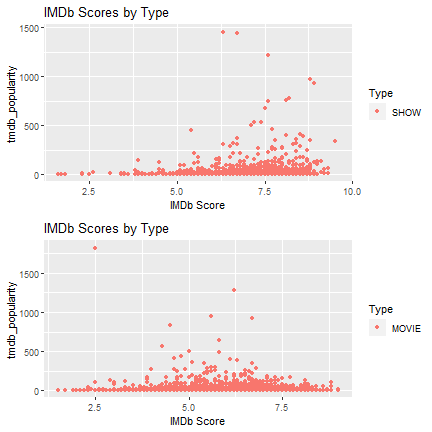
\includegraphics{Question-4_files/figure-latex/Figure 1-1} 

}

\caption{Show vs movie \label{Figure1}}\label{fig:Figure 1}
\end{figure}

\begin{verbatim}
## TableGrob (2 x 1) "arrange": 2 grobs
##   z     cells    name           grob
## 1 1 (1-1,1-1) arrange gtable[layout]
## 2 2 (2-2,1-1) arrange gtable[layout]
\end{verbatim}

From the above scatter plot \ref{Figure1}, it is evident that shows
outperform movies. Shows have higher overall scores and ratings. To
further ensure this scatter plot provides the correct interpretation, i
will next look at the averages in a table.

\hypertarget{table-to-compare-show-and-movie}{%
\subsection{Table to compare Show and
movie}\label{table-to-compare-show-and-movie}}

\begin{longtable}{cccc}
\caption*{
{\large Averages for show and movie}
} \\ 
\toprule
Type & Average\_Score & Average\_Popularity & Average\_Votes \\ 
\midrule
Show & $7.0$ & $30.6$ & $17,745.0$ \\ 
Movie & $6.3$ & $19.8$ & $27,097.4$ \\ 
\bottomrule
\end{longtable}

From the above table \ref{Figure2}, it is evident that the suspension
made by looking at \ref{Figure2} are correct. Shows do outperform
movies. Shows have a much higher popularity and a higher score. Thus it
seems to be that it would be more beneficial for a streaming service to
focus on TV shows over movies. Next I will be looking at which age
resiticted shows and movies are the most popular and highest rated.

\hypertarget{age-certification-plot}{%
\subsection{Age certification plot}\label{age-certification-plot}}

\begin{figure}[H]

{\centering 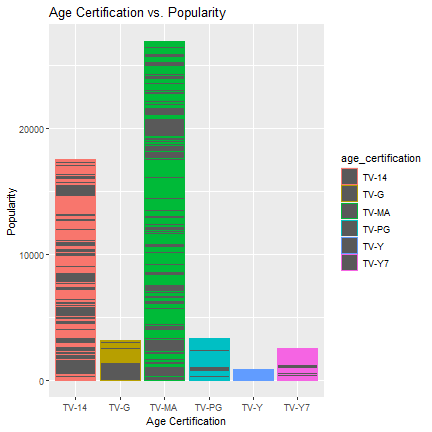
\includegraphics{Question-4_files/figure-latex/Figure 3-1} 

}

\caption{age certification \label{Figure3}}\label{fig:Figure 3}
\end{figure}

From the above figure \ref{Figure3}, it is evident that if a streaming
service wnats to put themselves in the best position to succeseed, they
should look at focusing on tv shows with a few movies with the age
certification of TV\_MA or TV-14.

\hypertarget{conclusion}{%
\section{Conclusion}\label{conclusion}}

After a short but thurough analysis it is suggested that if a streaing
service wants to learn from Netflex they should look at focusing on tv
shows with a few movies with the age certification of TV\_MA or TV-14.

\bibliography{Tex/ref}





\end{document}
